%
% The preamble, here we define packages and options for the article
%
\documentclass[11pt]{article}

% Set the paper size to A4 and the margins to 1in
\usepackage{geometry}
\geometry{
    a4paper,
    left=1in,
    right=1in,
    top=1in,
    bottom=1in
}

% Allow font specifications
\usepackage{fontspec}
% Allow multiple languages in the text
\usepackage{polyglossia}
\setdefaultlanguage{greek}
\setotherlanguage{english}
\setsansfont[
    Extension      = .ttf,
    UprightFont    = *,
    ItalicFont     = *i,
    BoldFont       = *b,
    BoldItalicFont = *z,
    Ligatures      = TeX,
    Path           = fonts/
]{cambria}
\setmonofont{Courier}
\newfontfamily{\greekfont}[
    Extension      = .ttf,
    UprightFont    = *,
    ItalicFont     = *i,
    BoldFont       = *b,
    BoldItalicFont = *z,
    Ligatures      = TeX,
    Path           = fonts/
]{cambria}
\newfontfamily{\greekfonttt}{Courier}
\newcommand*{\mytextvisiblespace}{\fontfamily{DejaVu}\selectfont\textvisiblespace}

\gappto\captionsgreek{
    \def\equationautorefname{Εξίσωση}
    \def\footnoteautorefname{υποσημείωση}
    \def\itemautorefname{στοιχείο}
    \def\figureautorefname{Σχήμα}
    \def\tableautorefname{Πίνακα}
    \def\partautorefname{Μέρος}
    \def\appendixautorefname{Παράρτημα}
    \def\chapterautorefname{Κεφάλαιο}
    \def\sectionautorefname{Eνότητα}
    \def\subsectionautorefname{Υποενότητα}
    \def\subsubsectionautorefname{Υπο-υποενότητα}
    \def\paragraphautorefname{Παράγραφο}
    \def\subparagraphautorefname{Υποπαράγραφο}
    \def\FancyVerbLineautorefname{γραμμή}
    \def\theoremautorefname{Θεώρημα}
    \def\pageautorefname{σελίδα}
    \def\lstlistingname{Κώδικας}
    \def\lstlistingautorefname{Κώδικας}
}

% Recomended for correct quotes
\usepackage{csquotes}

\newenvironment{alltt}{\ttfamily}{\rmfamily}

% Specify colors
\usepackage[dvipsnames]{xcolor}
\colorlet{mylinkcolor}{red!50!black}
\colorlet{mycitecolor}{YellowOrange}
\colorlet{myurlcolor}{MidnightBlue}

\usepackage{listings}
\lstset{numbers=left}
\lstset{showstringspaces=false}
\usepackage[framed]{matlab-prettifier}

% Add hyperlinks and refrences
\usepackage{hyperref}
\hypersetup{
    linkcolor  = mylinkcolor!85!black,
    citecolor  = mycitecolor!85!black,
    urlcolor   = myurlcolor!85!black,
    colorlinks = true,
    pdftitle   = {Ανεύρεση Κωδικού με Χρήση Μαρκοβιανών Αλυσίδων},
    pdfauthor  = {Χρήστος Γκαντίδης, Αναστασιάδου Μαγδαλινή}
}

% Draw a graph in LaTeX
\usepackage{tikz}
\usetikzlibrary{arrows}

% Display more advanced math
\usepackage{amsmath}
% Command to display variable names in upright font
\newcommand*{\var}[1]{\operatorname{#1}}

% Enter a vertical space between paragraphs instead of first line indentation
\usepackage{parskip}

% Display values with SI units beatifully
\usepackage{siunitx}
\sisetup{group-minimum-digits = 3}

% Make references take you not to the caption but the whole table/image
\usepackage{caption}

% Allow long tables to span multiple mages
\usepackage{longtable}

% Easily draw square arrays
\usepackage[thinlines]{easytable}

% Add images
\usepackage{graphicx}
\graphicspath{ {img/} }

% Bibliography
\usepackage[backend=biber,
            style=alphabetic,
            sorting=ynt]{biblatex}
\addbibresource{bibliography.bib}

% Set the title of the article
\title{
    Ανεύρεση Κωδικού με Χρήση Μαρκοβιανών Αλυσίδων \\[20pt]
    \large Ασφάλεια Συστημάτων Υπολογιστών \\
    Γεώργιος Δροσάτος
}

% Set the author of the article
\author{
    Αναστασιάδου Μαγδαλινή 56678
    \\ email: \href{mailto:magdanas@ee.duth.gr}{magdanas@ee.duth.gr}
    \and
    Γκαντίδης Χρήστος 56483 \\
    email: \href{mailto:chrigkan@ee.duth.gr}{chrigkan@ee.duth.gr}
}

\date{Δεκέμβριος 2017}

\begin{document}
\pagenumbering{gobble}
% Don't number first page
\maketitle

\newpage
\pagenumbering{roman}
\tableofcontents

\newpage
\pagenumbering{arabic}
\section{Περίληψη Μαρκοβιανών Αλυσίδων}

Οι Μαρκοβιανές αλυσίδες, οι οποίες παίρνουν το όνομά τους από τον Andrey Markov (1856-1922), είναι μαθηματικές κατασκευές οι οποίες περιγράφουν την μετάβαση ενός συστήματος από μια κατάσταση σε όλες τις υπόλοιπες δυνατές καταστάσεις του συστήματος \cite{wiki:markov_chain}.

Για παράδειγμα, ας θεωρήσουμε τον καιρό μιας περιοχής ως ένα σύστημα, με το σύστημα αυτό να έχεις τις δυνατές καταστάσεις \{\textit{λιακάδα}, \textit{συννεφιά}, \textit{βροχή}, \textit{χιόνι}, \textit{χαλάζι}\}, στις οποίες αναφερόμαστε ως \textit{πεδίο καταστάσεων}.

Επιπλέον, μπορούμε να ορίσουμε μια Μαρκοβιανή αλυσίδα, η οποία περιγράφει την πιθανότητα μετάβασης από την μια κατάσταση στην άλλη, για παράδειγμα από την κατάσταση \textit{λιακάδα} στην κατάσταση \textit{συννεφιά}. Ο πιο εύκολος τρόπος να αναπαραστήσουμε γραφικά μια Μαρκοβιανή αλυσίδα είναι σε μορφή γράφου όπως φαίνεται στο \autoref{fig:markov_chain_graph}.

\begin{figure}[h]
    \centering
    \begin{tikzpicture}
        [nstyle/.style={circle, draw=blue!50, fill=blue!20, thick, inner sep=0em, minimum size=6em},
        vstyle/.style={circle, fill=white},
        dstyle/.style={->, very thick}]
        
        \node[vstyle] (sunny1)  at (0,0) {0.7};
        \node[nstyle] (sunny)   at (2,0) {λιακάδα};
        \node[nstyle] (cloudy)   at (6,0) {συννεφιά};
        \node[vstyle] (cloudy1)  at (8,0) {0.6};
        
        \draw[dstyle] (sunny) to[bend left=45] node[circle,fill=white]{0.3} (cloudy);
        \draw[dstyle] (cloudy) to[bend left=45] node[circle,fill=white]{0.4} (sunny);
        \draw[very thick] (sunny) to[in=90, out=135] (sunny1);
        \draw[dstyle] (sunny1) to[in=225, out=270] (sunny);
        \draw[very thick] (cloudy) to[in=270, out=315] (cloudy1);
        \draw[dstyle] (cloudy1) to[in=45, out=90] (cloudy);
    \end{tikzpicture}
    \caption{Αναπαράσταση Μαρκοβιανής Αλυσίδας με Μορφή Γράφου.\label{fig:markov_chain_graph}}
\end{figure}


Για δύο δυνατές καταστάσεις, υπάρχουν τέσσερις δυνατές μεταβάσεις, καθώς από κάθε κατάσταση υπάρχει η πιθανότητα να μεταβούμε στην άλλη ή να παραμείνουμε στην ίδια. Γενικά για κάθε $n$ καταστάσεις υπάρχουν $n^2$ δυνατές μεταβάσεις.

Επειδή για μεγαλύτερα $n$ οι αναπαραστάσεις με μορφή γράφου αρχίζουν να γίνονται χαοτικές, προτιμούμε την αναπαράσταση των Μαρκοβιανών αλυσίδων ως έναν τετραγωνικό πίνακα $A$, με το $A[i,j]$ να αναπαριστά την πιθανότητα μετάβασης από την κατάσταση $i$ στην $j$, όπως φαίνεται στον \autoref{tab:markov_chain_table} \cite{setosa:markov_chain}.

\begin{table}[h]
    \centering
    \begin{TAB}(c){c|c|c|}{c|c|c|}
                    & λιακάδα   & συννεφιά  \\
        λιακάδα     & $0.7$     & $0.3$     \\
        συννεφιά    & $0.4$     & $0.6$     \\
    \end{TAB}
    \caption{Αναπαράσταση Μαρκοβιανής Αλυσίδας με Μορφή Πίνακα.\label{tab:markov_chain_table}}
\end{table}

Παρατηρούμε, και εξάγουμε εύκολα το συμπέρασμα, πως το άθροισμα των στοιχείων μιας γραμμής πρέπει να είναι $1$, όπως και η συνολική πιθανότητα μετάβασης.

Οι Μαρκοβιανές αλυσίδες είναι πολύ χρήσιμες για συστήματα τα οποία δεν μεταβαίνουν με την ίδια πιθανότητα σε όλες τις καταστάσεις, αλλά δείχνουν μια προτίμηση προς κάποιες από αυτές. Για το παραπάνω παράδειγμα, όταν μια μέρα έχει \textit{λιακάδα}, τότε η πιθανότητα να έχει και την επόμενη μέρα \textit{λιακάδα} είναι μεγαλύτερη από την πιθανότητα να έχει \textit{συννεφιά}. Έτσι η πιθανότητα μετάβασης από \textit{λιακάδα} σε \textit{λιακάδα} είναι μεγαλύτερη από την πιθανότητα μετάβασης από \textit{λιακάδα} σε \textit{συννεφιά}.

\section{Κατακερματισμός Κωδικών}

\subsection{Συναρτήσεις Κατακερματισμού}

Οι \textit{Συναρτήσεις Κατακερματισμού (hash functions)}, είναι συναρτήσεις οι οποίες δέχονται ως είσοδο δεδομένα οποιουδήποτε μεγέθους, και τα αντιστοιχίζουν ντετερμινιστικά σε κάποια άλλα δεδομένα σταθερού μεγέθους. Δεν πρόκειται για μεθόδους κρυπτογράφησης, καθώς δεν υπάρχει καθορισμένος τρόπος να μεταβούμε από τα δεδομένα εξόδου της συνάρτησης στα δεδομένα εισόδου. Έτσι, χρησιμοποιούνται για την επιβεβαίωση της ακεραιότητας των δεδομένων μετά από την μετάδοσή τους, ή για την επαλήθευση γνώσης των δεδομένων εισόδου \cite{wiki:hash_function}.

Μια από τις κύριες χρήσεις των Συναρτήσεων Κατακερματισμού, είναι η αποθήκευση κωδικών των χρηστών μιας σελίδας, σε μια βάση δεδομένων, με στόχο την προστασία των προσωπικών δεδομένων των χρηστών. Έτσι, σε περίπτωση που η βάση δεδομένων διαρρεύσει και αποκτήσουν πρόσβαση σε αυτήν τρίτοι, οι κωδικοί δεν βρίσκονται σε μορφή \textit{απλού κειμένου (plain text)}, και οι τρίτοι δεν μπορούν να χρησιμοποιήσουν τους κωδικούς για να αποκτήσουν πρόσβαση σε λογαριασμούς των χρηστών σε άλλες σελίδες \cite{crackstation:password_hashing}.

Μια από τις πιο γνωστές και ευρέως χρησιμοποιούμενη Συνάρτηση Κατακερματισμού, η οποία όμως δεν θεωρείται πλέον κρυπτογραφικά ασφαλής, είναι η MD5 \cite{wiki:md5}. Δέχεται ως είσοδο ένα μπλοκ δεδομένων, που στην δική μας περίπτωση είναι ο κωδικός απλού κειμένου, και παράγει στην έξοδό της μια τιμή \SI{128}{bits}, δηλαδή \SI{16}{Bytes}, η οποία αναπαριστάται συνήθως από \SI{32} δεκαεξαδικούς χαρακτήρες. Η έξοδος της MD5 αλλάζει δραματικά, ακόμα και με μια μικρή αλλαγή στην είσοδο της, όπως φαίνεται στον \autoref{tab:md5_hash_in_out}.

\begin{table}[h]
    \centering
    \begin{alltt}
        \begin{TAB}(r){l|r}{c|ccc}
            \rmfamily{κωδικός}       & \rmfamily{MD5 hash} \\
            apple                    & 1f3870be274f6c49b3e31a0c6728957f \\
            Apple                    & 9f6290f4436e5a2351f12e03b6433c3c \\
            apple\mytextvisiblespace & e307c4bc0265c934316dbd59f86336fd \\
        \end{TAB}
    \end{alltt}
    \caption{Μια μικρή μεταβολή της εισόδου, προκαλεί μεγάλη μεταβολή της εξόδου.\label{tab:md5_hash_in_out}}
\end{table}

Λόγω του ότι οι Συναρτήσεις Κατακερματισμού δεν μπορούν να αντιστραφούν, δεν μπορούμε δηλαδή να παράγουμε την είσοδο από την έξοδο, οι μόνοι τρόποι να βρούμε ποιος κωδικός απλού κειμένου αντιστοιχεί στον κωδικό κατακερματισμού, είναι είτε να γνωρίζουμε εξαρχής τον κωδικό απλού κειμένου (επαλήθευση γνώσης των δεδομένων εισόδου), είτε να δοκιμάσουμε όλους του δυνατούς κωδικούς απλού κειμένου ως εισόδους της Συνάρτησης Κατακερματισμού μέχρι να βρούμε την έξοδο που είναι ίδια με τον κατακερματισμένο κωδικό, οπότε και έχουμε βρει τον ζητούμενο κωδικό απλού κειμένου. Η διαδικασία αυτή λέγεται \textit{Ανεύρεση Κωδικού (Password Guessing/Cracking)} \cite{wiki:password_cracking} και θα περιγραφεί παρακάτω.

\subsection{Ανεύρεση Κωδικού Απλού Κειμένου από Κατακερματισμένο Κωδικό}

Οι σελίδες που αποθηκεύουν τους κωδικούς των χρηστών τους σε κατακερματισμένη μορφή, επαληθεύουν πως ο χρήστης που προσπαθεί να εισέλθει είναι αυτός που δημιούργησε τον λογαριασμό, περνώντας τον κωδικό απλού κειμένου που εισήγαγε στην σελίδα εισόδου από την συνάρτηση κατακερματισμού, και ελέγχοντας αν το αποτέλεσμα είναι ίδιο με την τιμή που υπάρχει αποθηκευμένη στην βάση. Σε περίπτωση που είναι ίδιο, τότε ο χρήστης είχε γνώση των αρχικών δεδομένων, δηλαδή του κωδικού απλού κειμένου που όρισε όταν δημιούργησε τον λογαριασμό του στην σελίδα, και έτσι του επιτρέπεται η πρόσβαση.

Παρακάτω, παρουσιάζουμε μια μέθοδο για την ανεύρεση του κωδικού απλού κειμένου, όταν δεν έχουμε δηλαδή από πριν γνώση των αρχικών δεδομένων, αλλά μόνο του κατακερματισμένου κωδικού. Αν και παρόμοιες μέθοδοι μπορούν να χρησιμοποιηθούν από κακόβουλους χρήστες, με σκοπό για παράδειγμα την πρόσβαση σε κάποιον άλλο λογαριασμό του χρήστη με τον ίδιο κωδικό απλού κειμένου, ο λόγος που παρουσιάζουμε την μέθοδο εμείς είναι ερευνητικός, και με απώτερο σκοπό να ευαισθητοποιήσουμε τους χρήστες ώστε να επιλέγουν κατάλληλους κωδικούς, οι οποίοι δεν είναι ευάλωτοι σε αυτού του είδους τις επιθέσεις.

\section{Μέθοδοι Ανεύρεσης}

\subsection{Μέθοδος Ωμής Βίας (Brute Force)}

Ο πιο απλός τρόπος για την ανεύρεση ενός κωδικού, είναι η επίθεση ωμής βίας \cite{wiki:brute_force_attack}, κατά την οποία δοκιμάζουμε όλους τους πιθανούς συνδυασμούς των χαρακτήρων που ανήκουν στο \textit{πεδίο χαρακτήρων (character space)}, συνήθως κατά αύξουσα σειρά.

Αν υποθέσουμε πως το πεδίο χαρακτήρων αποτελείται από όλους τους πεζούς χαρακτήρες (a--z), και θέλουμε να δοκιμάσουμε όλους τους κωδικούς με μήκος τρεις χαρακτήρες, τότε η μέθοδος ωμής βίας θα δοκιμάσει τους κωδικούς με την σειρά που φαίνεται στον \autoref{tab:bruteforce}.

\begin{table}[h]
    \centering
    \begin{alltt}
        \begin{tabular}{ccccccc}
            aaa & aba & $\cdots$ & baa & bba & $\cdots$ & zza \\
            aab & abb & $\cdots$ & bab & bbb & $\cdots$ & zzb \\
            aac & abc & $\cdots$ & bac & bbc & $\cdots$ & zzc \\
            $\vdots$ & $\vdots$ & $\ddots$ & $\vdots$ & $\vdots$ & $\ddots$ & $\vdots$ \\
            aaz & abz & $\cdots$ & baz & bbz & $\cdots$ & zzz \\
        \end{tabular}
    \end{alltt}
    \caption{Παράδειγμα εκτέλεση μεθόδου ωμής βίας.\label{tab:bruteforce}}
\end{table}

Στην πραγματικότητα, και στο παρόν έργο, το πεδίο χαρακτήρων αποτελείται συνήθως από όλους τους εκτυπώσιμους χαρακτήρες του κώδικα ASCII (κωδικοί 32--126) \cite{wiki:graphic_character_ascii}:
\begin{alltt}
    \begin{description}
        \item[lowercase] a, b, c, d, e, f, g, h, i, j, k, l, m, n, o, p, q, r, s, t, u, v, w, x, y, z
        \item[upercase] A, B, C, D, E, F, G, H, I, J, K, L, M, N, O, P, Q, R, S, T, U, V, W, X, Y, Z
        \item[numbers] 0, 1, 2, 3, 4, 5, 6, 7, 8, 9
        \item[punctuation] \mytextvisiblespace (space), !, ", \#, \$, \%, \&, ', (, ), *, +, ,, -, ., /, :, ;, <, =, >, ?, @, [, \textbackslash, ], \textasciicircum, \_, `, \{, |, \}, \textasciitilde
    \end{description}
\end{alltt}

Σε πιο επαγγελματικές βάσεις δεδομένων και για σελίδες με διεθνές κοινό (που έχουν χρήστες για παράδειγμα και στην Ασία), μπορεί να χρησιμοποιηθούν όλοι οι εκτυπώσιμοι χαρακτήρες του κώδικα Unicode \cite{wiki:graphic_character_unicode} κάτι που ξεφύγει όμως από το πεδίου αυτού του έργου.

Όπως ίσως είναι εύκολο να αντιληφθεί κανείς, αν το μήκος του κωδικού απλού κειμένου είναι $n$ χαρακτήρες, και το πεδίο χαρακτήρων αποτελείται από $s$ χαρακτήρες, θα πρέπει να δοκιμάσουμε $s^n$ διαφορετικούς κωδικούς. Η μέθοδος ωμής βίας δηλαδή έχει υπολογιστική πολυπλοκότητα $\mathcal{O}(s^n)$.

\subsection{Μέθοδος Λεξικού (Dictionary)}
\label{subsec:dictionary}

Η μέθοδος λεξικού (dictionary attack) βασίζεται στην δοκιμή λέξεων από μια υπάρχουσα λίστα. Σε αντίθεση με την μέθοδο ωμής βίας, η μέθοδος λεξικού περιορίζεται μόνο σε συνηθισμένες ακολουθίες χαρακτήρων που είναι εύκολο να απομνημονευθούν. Η επιτυχία της οφείλεται στο γεγονός ότι πολλοί χρήστες επιλέγουν μικρούς σε μέγεθος κωδικούς, οι οποίοι είναι είτε μια καθημερινή λέξη είτε απλή παραλλαγή μιας λέξης, όπως για παράδειγμα την μετατροπή κάποιων χαρακτήρων από πεζούς σε κεφαλαίους, την προσθήκη κάποιου αριθμού στο τέλος της λέξης, την αντικατάσταση κάποιων χαρακτήρων με κάποια σύμβολα (l33t-speak) ή κάποιον συνδυασμό των παραπάνω \cite{wiki:dictionary_attack}.

Για παράδειγμα, ένας κωδικός πεζών χαρακτήρων, με μήκος οκτώ, με την μέθοδο ωμής βίας θα χρειαζόταν στην χειρότερη περίπτωση $26 \cdot 26 \cdot 26 \cdot 26 \cdot 26 \cdot 26 \cdot 26 \cdot 26 = 26^8$  προσπάθειες για να εντοπιστεί. Με έναν ρυθμό δοκιμής \SI{5000000} κωδικών το δευτερόλεπτο (ρυθμός που πετυχαίνεται εύκολα από σύγχρονο υλικό), θα απαιτούνταν περίπου \SI{11.6}{h}.

Από την άλλη μεριά, ο αριθμός των λέξεων στο Oxford English Dictionary είναι περίπου \SI{600000}, θεωρώντας ότι ο μέσος άνθρωπος χρησιμοποιεί ένα μόνο μέρος αυτών των λέξεων, από \SI{10000} έως \SI{40000}, θα απαιτούνταν γύρω στα \SI{8}{ms} για να δοκιμαστούν όλες οι λέξεις!

Ακόμη, είναι σχετικά εύκολο ο επιτιθέμενος να δημιουργήσει και να αποθηκεύσει μια λίστα με κατακερματισμένους κωδικούς από όλες τις λέξεις σε ένα λεξικό. Εάν γνωρίζει τον κατακερματισμένο κωδικό κάποιου τότε μπορεί σχεδόν ακαριαία να τον αναζητήσει και να τον εντοπίσει στην λίστα που δημιούργησε.

Αν το λεξικό περιέχει $l$ λέξεις, τότε η μέθοδος λεξικού θα δοκιμάσει $l$ διαφορετικούς κωδικούς, έχει δηλαδή υπολογιστική πολυπλοκότητα $\mathcal{O}(l)$. Αν και πρόκειται για σημαντική βελτίωση από την εκθετική πολυπλοκότητα της μεθόδου ωμής βίας, είναι αρκετά περιορισμένη από το μήκος του λεξικού, και από το γεγονός πως μπορεί ο κωδικός να μην βρίσκεται μέσα σε κανένα λεξικό.

\subsection{Μέθοδος με Χρήση Μαρκοβιανών Αλυσίδων (Markov Chains)}
\label{subsec:markov_chains}

Με την χρήση των Μαρκοβιανών αλυσίδων, μπορούμε να βελτιώσουμε την μέθοδο ωμής βίας \cite{trustwave:hashcat_per_position_markov_chains}. Η όλη λογική βασίζεται στο γεγονός ότι στις λέξεις της φυσική γλώσσας, η συχνότητα και η ακολουθία των γραμμάτων δεν είναι ισοπίθανη.

Ένα παράδειγμα που δείχνει την διαφορά στην συχνότητα των χαρακτήρων στην Αγγλική γλώσσα\footnotemark, είναι το ότι υπάρχουν περισσότερες λέξεις που ξεκινάνε με τον χαρακτήρα \texttt{'c'} παρά με τον χαρακτήρα \texttt{'b'}. Έτσι, είναι λογικό, όταν προσπαθούμε να βρούμε τον κωδικό απλού κειμένου, να δοκιμάσουμε όλους τους κωδικούς που ξεκινάνε με \texttt{'c'} πριν αυτούς που ξεκινάνε με \texttt{'b'}, και όχι με καθαρά αλφαβητική σειρά, καθώς υπάρχει μεγαλύτερη πιθανότητα να βρούμε τον σωστό κωδικό στην πρώτη περίπτωση, γλιτώνοντας έτσι πολύτιμο χρόνο και υπολογιστικό έργο.

Ένα άλλο παράδειγμα, που δείχνει αυτή τη φορά την διαφορά στην ακολουθία των χαρακτήρων στην Αγγλική γλώσσα\footnotemark[\value{footnote}], είναι το ότι υπάρχουν περισσότερες περιπτώσεις κατά τις οποίες ο χαρακτήρας \texttt{'a'} ακολουθείται από τον χαρακτήρα \texttt{'b'}, παρά από τον χαρακτήρα \texttt{'a'}. Και πάλι, είναι λογικό, όταν ο προηγούμενος χαρακτήρας του κωδικού είναι \texttt{'a'}, να δοκιμάσουμε στην τωρινή θέση τον χαρακτήρα \texttt{'b'} πριν από τον χαρακτήρα \texttt{'a'}, και όχι με καθαρά αλφαβητική σειρά, τακτική που μας επιφέρει και πάλι τα κέρδη που περιγράφηκαν πριν.

Το παραπάνω παράδειγμα αποκτά ακόμα μεγαλύτερη ισχύ, αν σκεφτούμε πως η ακολουθία των χαρακτήρων αλλάζει ανάλογα με την θέση μέσα στην λέξη\footnotemark[\value{footnote}]. Έτσι, στην δεύτερη θέση, είναι πιο πιθανό ο χαρακτήρας \texttt{'a'} να ακολουθείται από τον χαρακτήρα \texttt{'s'} παρά από τον χαρακτήρα \texttt{'t'}. Οι πιθανότητες αυτές όμως αντιστρέφονται στην τρίτη θέση της λέξης, όπου ο χαρακτήρας \texttt{'a'} είναι πιο πιθανό να ακολουθείται από τον χαρακτήρα \texttt{'t'} παρά από τον χαρακτήρα \texttt{'s'}.

\footnotetext{Σύμφωνα με το λεξικό \texttt{/usr/share/dict/american-english} που βρίσκεται σε όλα τα λειτουργικά *nix}

Εκμεταλλευόμαστε τις παραπάνω ιδιαιτερότητες με την χρήση των Μαρκοβιανών αλυσίδων, ώστε να δοκιμάζουμε τους πιθανούς κωδικούς απλού κειμένου κατά φθίνουσα πιθανότητα εμφάνισης των χαρακτήρων στην αντίστοιχη θέση, ανάλογα με τον χαρακτήρα στην θέση που προηγείται.

Ένα ακόμα προτέρημα έναντι της μεθόδου ωμής βίας, είναι ότι μπορούμε να περιορίσουμε την πολυπλοκότητα του αλγορίθμου, ορίζοντας ένα όριο στο πλήθος των διαφορετικών χαρακτήρων που θα δοκιμαστούν σε κάθε θέση. Μπορούμε για παράδειγμα να δοκιμάσουμε μόνο τους 30 πιο πιθανούς χαρακτήρες σε κάθε θέση, έναντι του να δοκιμάσουμε όλους τους 95 δυνατούς χαρακτήρες.

Για παράδειγμα, αν το μήκος του κωδικού απλού κειμένου είναι $n$ χαρακτήρες, και το πεδίο χαρακτήρων έχει πληθικότητα $s$, μπορούμε να ορίσουμε ένα \textit{όριο (threshold)} $t; t \le s$, έχοντας έτσι να δοκιμάσουμε $t^n$ αντί για $s^n$ διαφορετικούς κωδικούς. Φαίνεται λοιπόν, πως η υπολογιστική πολυπλοκότητα της μεθόδου Μαρκοβιανών αλυσίδων είναι $\mathcal{O}(t^n)$, με την δυνατότητα να κάνουμε το $t$ όσο μικρό θέλουμε. Σε περίπτωση που $t=s$, τότε η μέθοδος Μαρκοβιανών αλυσίδων εκφυλλίζεται στην μέθοδο ωμής βίας, με το πλεονέκτημα της σειράς με την οποία θα δοκιμαστούν οι κωδικοί όμως να παραμένει.

\subsection{Ιριδίζοντες Πίνακες (Rainbow Tables)}

Οι ιριδίζοντες πίνακες έρχονται να μετατρέψουν το φορτίο, από υπολογιστικό σε αποθηκευτικό. Αντί να παράγουμε κάθε φορά τους κατακερματισμένους κωδικούς που αντιστοιχούν στους κωδικούς απλού κειμένου, μπορούμε να τους αποθηκεύσουμε μαζί σε ένα αρχείο, και αργότερα να πραγματοποιήσουμε απλά μια αναζήτηση για να εντοπίσουμε τον κωδικό απλού κειμένου που αντιστοιχεί στον κατακερματισμένο κωδικό. Η τακτική αυτή υπάρχει εδώ και πολλά χρόνια, και έχει χρησιμοποιηθεί με επιτυχία \cite{wiki:rainbow_table}, αλλά έχει ένα βασικό μειονέκτημα: περιορίζεται από το μήκος του κωδικού.

Αν υποθέσουμε πως το πεδίο χαρακτήρων αποτελείται από τους 95 εκτυπώσιμους χαρακτήρες του κώδικα ASCII, πως κάθε χαρακτήρας αναπαριστάται από \SI{8}{bits}, και θυμηθούμε πως το αποτέλεσμα της συνάρτηση κατακερματισμού MD5 είναι μια τιμή \SI{128}{bits}, τότε στον \autoref{tab:file_sizes} παρουσιάζονται τα μεγέθη των αρχείων που απαιτούνται για να αποθηκεύσουν τα ζεύγη κατακερματισμένου κωδικού και κωδικού απλού κειμένου. Όπως βλέπουμε το μέγεθος των αρχείων αυξάνεται εκθετικά.

\begin{table}[h]
    \centering
    \begin{tabular}{r|r|r}
        \# χαρακτήρων & \# πιθανών κωδικών & μέγεθος αρχείου \\\hline
        \SI{1} & \SI{95} ($10^{1.98}$) & \SI{1.58}{KiB} \\
        \SI{2} & \SI{9025} ($10^{3.96}$) & \SI{158.64}{KiB} \\
        \SI{3} & \SI{857375} ($10^{5.93}$) & \SI{15.54}{MiB} \\
        \SI{4} & \SI{81450625} ($10^{7.91}$) & \SI{1.52}{GiB} \\
        \SI{5} & \SI{7737809375} ($10^{9.89}$) & \SI{151.33}{GiB} \\
        \SI{6} & \SI{735091890625} ($10^{11.87}$) & \SI{14.71}{TiB} \\
        \SI{7} & \SI{69833729609375} ($10^{13.84}$) & \SI{1.43}{PiB} \\
        \SI{8} & \SI{6634204312890625} ($10^{15.82}$) & \SI{141.42}{PiB} \\
        \SI{9} & \SI{630249409724609375} ($10^{17.80}$) & \SI{13.67}{EiB} \\
    \end{tabular}
    \caption{Μέγεθος αρχείου αποθήκευσης Ιριδίζοντος Πίνακα. \label{tab:file_sizes}}
\end{table}

Η μέθοδος βέβαια καθίσταται σχεδόν αδύνατη σε περιπτώσεις που οι κωδικοί είναι αποθηκευμένοι μαζί με κάποιο μεγάλου μήκους τυχαία ακολουθία χαρακτήρων, που ονομάζεται \textit{salt}. Δηλαδή όταν ο κατακερματισμένος κωδικός που γνωρίζει εκ των προτέρων ο επιτιθέμενος δεν προέκυψε απλά από το αποτέλεσμα της συνάρτησης κατακερματισμού για τον κωδικό του χρήστη, αλλά από το αποτέλεσμα αυτής της συνάρτησης για την συνένωση του κωδικού του χρήστη με το salt.

\begin{table}[h]
    \centering
    \begin{TAB}(r){l|r|r}{c|cccc}
        κωδικός & salt & MD5 hash \\
        \texttt{hello}   & \texttt{-}              & \texttt{5d41402abc4b2a76b9719d911017c592} \\
        \texttt{hello}   & \texttt{QxLUF1bgIAdeQX} & \texttt{61819a2e9b721831243eba1aeaba8486} \\
        \texttt{hello}   & \texttt{bv5PehSMfV11Cd} & \texttt{3c3fbfc82061e60fb6c11a5e0307058e} \\
        \texttt{hello}   & \texttt{YYLmfY6IehjZMQ} & \texttt{104f4f46d8222b57cbd543d75a3b8947} \\
    \end{TAB}
    \caption{Αποτέλεσμα της συνάρτησης κατακερματισμού MD5 με χρήση salt.\label{tab:MD5_saltedhash}}
\end{table}

Σε μια τέτοια περίπτωση, χρήστες με τον ίδιο κωδικό δεν θα είχαν τους ίδιους κατακερματισμένους κωδικούς, όπως φαίνεται στον \autoref{tab:MD5_saltedhash}. Ο επιτιθέμενος θα έπρεπε τότε να παράγει και να αποθηκεύσει τους ιριδίζοντες πίνακες που προκύπτουν για κάθε salt συνδυασμένο με κάθε δυνατή λέξη που δημιουργείται με $n$ χαρακτήρες. Οι συνδυασμοί συνεπώς πολλαπλασιάζονται, και η αποθήκευση ενός τέτοιου πίνακα είναι πρακτικά αδύνατη.

\section{Υλοποίηση Μεθόδου Μαρκοβιανών Αλυσίδων}

Ο πηγαίος κώδικας που υλοποιεί την μέθοδο Μαρκοβιανών αλυσίδων όπως παρουσιάζεται στο παρόν έργο, μπορεί να βρεθεί στο GitHub στην διεύθυνση \url{https://github.com/christosg88/markov_guessing}.

\subsection{Παραγωγή Μαρκοβιανών Πινάκων}

Αφού είδαμε στις προηγούμενες ενότητες την χρησιμότητα των Μαρκοβιανών αλυσίδων στην ανεύρεση κωδικών και τα προτερήματά τους σε σχέση με άλλες μεθόδους, ας δούμε τώρα πώς υλοποιούνται.

Στο παρόν έργο δημιουργείται ένας Μαρκοβιανός πίνακας για κάθε θέση του κωδικού (per position Markov table), με σκοπό να εκμεταλλευτούμε την συνολική ισχύ που μας προσφέρουν, όπως περιγράφηκε στην \autoref{subsec:markov_chains}.

Σημαντικό παράγοντα στην ποιότητα των παραγόμενων πινάκων έχει η λίστα των λέξεων από την οποία εξάγουμε τις συχνότητες και τις ακολουθίες των χαρακτήρων. Αν για παράδειγμα χρησιμοποιούσαμε ένα απλό λεξικό της Αγγλικής γλώσσας, τότε οι Μαρκοβιανοί πίνακες θα ήταν πολύ καλοί στο να παράγουν λέξεις της Αγγλική γλώσσας. Εμείς όμως θέλουμε να χρησιμοποιήσουμε τους πίνακες για να παράγουμε πραγματικούς κωδικούς, που όπως είδαμε στην \autoref{subsec:dictionary} μπορεί να έχουν στο τέλος της λέξης διάφορους αριθμούς ή χαρακτήρες στίξης, ή άλλες μετατροπές.

Ο κώδικας έχει γραφεί με τέτοιον τρόπο, ώστε οι Μαρκοβιανοί πίνακες να μπορούν να παραχθούν από οποιαδήποτε λίστα κωδικών απλού κειμένου \textit{(wordlist)}. Φυσικά όσο πιο γενική είναι η λίστα και όσους περισσότερους κωδικούς απλού κειμένου περιέχει, τόσο πιο αποδοτικοί θα είναι οι πίνακες. Αφήνεται στην ηθική κρίση του αναγνώστη το πού θα βρει μια τέτοια λίστα και αν θα την χρησιμοποιήσει, καθώς αυτές οι λίστες στην πλειοψηφία τους προέρχονται από διαρρεύσεις βάσεων δεδομένων σελίδων που δεν κράτησαν με επιτυχία ασφαλείς τους κωδικούς των χρηστών τους.

Στο παρόν έργο περιορίσαμε τους κωδικούς σε μήκος μέχρι 10 χαρακτήρες, αλλά αυτό μπορεί εύκολα να αλλάξει με μια μικρή μετατροπή σε μια σταθερά στον πηγαίο κώδικα. Επίσης, θεωρήσαμε ως πεδίο χαρακτήρων το πλήρες διάστημα εκτυπώσιμων χαρακτήρων του πίνακα ASCII (κωδικοί 32--126), με πληθικότητα 95. Αφού από κάθε μια κατάσταση (προηγούμενος χαρακτήρας), μπορούμε να πάμε σε οποιαδήποτε κατάσταση (τρέχων χαρακτήρας), δημιουργούμε έναν πίνακα με διαστάσεις 95$\times$95 για κάθε θέση, δηλαδή 10 στο πλήθος.

Για την πρώτη θέση του κωδικού, καθώς δεν προηγείται από κανέναν χαρακτήρα, χρησιμοποιήσαμε μόνο την συχνότητα των χαρακτήρων που εμφανίζονται στην θέση αυτή, καθώς η λογική της ακολουθίας δεν ορίζεται. Οι συχνότητες αυτές αποθηκεύτηκαν στην πρώτη γραμμή του Μαρκοβιανού πίνακα για την θέση αυτή.

Μια μικρή μετατροπή που εφαρμόσαμε στους πίνακες, είναι πως δεν χρησιμοποιήσαμε την \textit{πιθανότητα} μετάβασης από τον έναν χαρακτήρα στον άλλο, αλλά την \textit{συχνότητα} μετάβασης. Έτσι, στους πίνακες αυτούς, οι γραμμές δεν αθροίζονται στην μονάδα. Με αυτόν τον τρόπο όμως εξοικονομούμε υπολογιστικό κόστος, καθώς δεν χρειάζεται να διαιρέσουμε την εκάστοτε συχνότητα με το πλήθος όλων των κωδικών για να βρούμε την πιθανότητα μετάβασης. Το μόνο που χρειαζόμαστε από τους πίνακες αυτούς είναι η φθίνουσα ταξινόμηση των χαρακτήρων, η οποία είναι η ίδια είτε χρησιμοποιήσουμε τις πιθανότητες ή τις συχνότητες.

Ο τρόπος που αναπαριστώνται αυτοί οι πίνακες στην μνήμη, είναι υπό την μορφή ενός τρισδιάστατου πίνακα (με όνομα $\var{markov}$ στο παράδειγμα που ακολουθεί), με μήκος πρώτης διάστασης το μέγιστο μήκος κωδικού (4 στο παράδειγμα), και μήκος δεύτερης και τρίτης διάστασης την πληθικότητα του πεδίου χαρακτήρων (5 στο παράδειγμα). Έτσι, για κάθε μια από τις θέσεις του κωδικού με μέγιστο μήκος, έχουμε έναν τετραγωνικό πίνακα που κρατάει τις συχνότητες εμφάνισης των χαρακτήρων.

Για να παραχθούν οι Μαρκοβιανοί πίνακες, αρχικοποιούμε όλες τις συχνότητες στο 0. Έπειτα, διατρέχουμε όλη την λίστα με τους κωδικούς που δίνεται ως είσοδος στο πρόγραμμα. Για κάθε κωδικό, ξεκινάμε από τον πρώτο χαρακτήρα (έστω $s_0$) και αυξάνουμε κατά 1 την τιμή στην θέση markov[$0$][$0$][$s_0$]. Συνεχίζουμε στον δεύτερο χαρακτήρα (έστω $s_1$) και αυξάνουμε κατά 1 την τιμή στην θέση markov[$1$][$s_0$][$s_1$]. Συνεχίζουμε για κάθε χαρακτήρα $s_i$ μέχρι τον τελευταίο, αυξάνοντας σε κάθε περίπτωση κατά 1 την τιμή στην θέση markov[$i$][$s_{i-1}$][$s_i$].

Ας δούμε ένα παράδειγμα παραγωγής πινάκων για να γίνει καλύτερα αντιληπτή η διαδικασία. Θα υποθέσουμε πως το πεδίο χαρακτήρων είναι το \{a, b, c, d, e\} και η λίστα με τους κωδικούς φαίνεται στον \autoref{tab:passwords}, με μέγιστο μήκος κωδικού 4.

\begin{table}[h]
    \centering
    \begin{alltt}
        \begin{tabular}{ll}
                ace & bee \\
                add & cab \\
                bad & dad \\
                bed & dead \\
        \end{tabular}
    \end{alltt}
    \caption{Παράδειγμα λίστας με κωδικούς. \label{tab:passwords}}
\end{table}

Οι πίνακες που παράγονται, και η παραγωγή τους Βήμα προς Βήμα φαίνονται στον \autoref{tab:markov_tables}.

\begin{frame}{Παράδειγμα}
    \only<1> {
        \begin{block}{Βήμα 0: Αρχικοποίηση}
            \begin{TAB}(c){cccc}{cc}
                \begin{TAB}(e)[3pt]{|c:c:c:c:c|}{|c:c:c:c:c|}
                    0 & 0 & 0 & 0 & 0 \\
                    0 & 0 & 0 & 0 & 0 \\
                    0 & 0 & 0 & 0 & 0 \\
                    0 & 0 & 0 & 0 & 0 \\
                    0 & 0 & 0 & 0 & 0 \\
                \end{TAB}
                &
                \begin{TAB}(e)[3pt]{|c:c:c:c:c|}{|c:c:c:c:c|}
                    0 & 0 & 0 & 0 & 0 \\
                    0 & 0 & 0 & 0 & 0 \\
                    0 & 0 & 0 & 0 & 0 \\
                    0 & 0 & 0 & 0 & 0 \\
                    0 & 0 & 0 & 0 & 0 \\
                \end{TAB}
                &
                \begin{TAB}(e)[3pt]{|c:c:c:c:c|}{|c:c:c:c:c|}
                    0 & 0 & 0 & 0 & 0 \\
                    0 & 0 & 0 & 0 & 0 \\
                    0 & 0 & 0 & 0 & 0 \\
                    0 & 0 & 0 & 0 & 0 \\
                    0 & 0 & 0 & 0 & 0 \\
                \end{TAB}
                &
                \begin{TAB}(e)[3pt]{|c:c:c:c:c|}{|c:c:c:c:c|}
                    0 & 0 & 0 & 0 & 0 \\
                    0 & 0 & 0 & 0 & 0 \\
                    0 & 0 & 0 & 0 & 0 \\
                    0 & 0 & 0 & 0 & 0 \\
                    0 & 0 & 0 & 0 & 0 \\
                \end{TAB}

                \\

                markov[$0$] & markov[$1$] & markov[$2$] & markov[$3$]
            \end{TAB}
        \end{block}
    }

    \only<2> {
        \begin{block}{Βήμα 1: ace}
            \begin{TAB}(c){cccc}{cc}
                \begin{TAB}(e)[3pt]{|c:c:c:c:c|}{|c:c:c:c:c|}
                    \textcolor{red}{1} & 0 & 0 & 0 & 0 \\
                    0 & 0 & 0 & 0 & 0 \\
                    0 & 0 & 0 & 0 & 0 \\
                    0 & 0 & 0 & 0 & 0 \\
                    0 & 0 & 0 & 0 & 0 \\
                \end{TAB}
                &
                \begin{TAB}(e)[3pt]{|c:c:c:c:c|}{|c:c:c:c:c|}
                    0 & 0 & \textcolor{red}{1} & 0 & 0 \\
                    0 & 0 & 0 & 0 & 0 \\
                    0 & 0 & 0 & 0 & 0 \\
                    0 & 0 & 0 & 0 & 0 \\
                    0 & 0 & 0 & 0 & 0 \\
                \end{TAB}
                &
                \begin{TAB}(e)[3pt]{|c:c:c:c:c|}{|c:c:c:c:c|}
                    0 & 0 & 0 & 0 & 0 \\
                    0 & 0 & 0 & 0 & 0 \\
                    0 & 0 & 0 & 0 & \textcolor{red}{1} \\
                    0 & 0 & 0 & 0 & 0 \\
                    0 & 0 & 0 & 0 & 0 \\
                \end{TAB}
                &
                \begin{TAB}(e)[3pt]{|c:c:c:c:c|}{|c:c:c:c:c|}
                    0 & 0 & 0 & 0 & 0 \\
                    0 & 0 & 0 & 0 & 0 \\
                    0 & 0 & 0 & 0 & 0 \\
                    0 & 0 & 0 & 0 & 0 \\
                    0 & 0 & 0 & 0 & 0 \\
                \end{TAB}

                \\

                markov[$0$] & markov[$1$] & markov[$2$] & markov[$3$]
            \end{TAB}
        \end{block}
    }

    \only<3> {
        \begin{block}{Βήμα 2: add}
            \begin{TAB}(c){cccc}{cc}
                \begin{TAB}(e)[3pt]{|c:c:c:c:c|}{|c:c:c:c:c|}
                    \textcolor{red}{2} & 0 & 0 & 0 & 0 \\
                    0 & 0 & 0 & 0 & 0 \\
                    0 & 0 & 0 & 0 & 0 \\
                    0 & 0 & 0 & 0 & 0 \\
                    0 & 0 & 0 & 0 & 0 \\
                \end{TAB}
                &
                \begin{TAB}(e)[3pt]{|c:c:c:c:c|}{|c:c:c:c:c|}
                    0 & 0 & 1 & \textcolor{red}{1} & 0 \\
                    0 & 0 & 0 & 0 & 0 \\
                    0 & 0 & 0 & 0 & 0 \\
                    0 & 0 & 0 & 0 & 0 \\
                    0 & 0 & 0 & 0 & 0 \\
                \end{TAB}
                &
                \begin{TAB}(e)[3pt]{|c:c:c:c:c|}{|c:c:c:c:c|}
                    0 & 0 & 0 & 0 & 0 \\
                    0 & 0 & 0 & 0 & 0 \\
                    0 & 0 & 0 & 0 & 1 \\
                    0 & 0 & 0 & \textcolor{red}{1} & 0 \\
                    0 & 0 & 0 & 0 & 0 \\
                \end{TAB}
                &
                \begin{TAB}(e)[3pt]{|c:c:c:c:c|}{|c:c:c:c:c|}
                    0 & 0 & 0 & 0 & 0 \\
                    0 & 0 & 0 & 0 & 0 \\
                    0 & 0 & 0 & 0 & 0 \\
                    0 & 0 & 0 & 0 & 0 \\
                    0 & 0 & 0 & 0 & 0 \\
                \end{TAB}

                \\

                markov[$0$] & markov[$1$] & markov[$2$] & markov[$3$]
            \end{TAB}
        \end{block}
    }

    \only<4> {
        \begin{block}{Βήμα 3: bad}
            \begin{TAB}(c){cccc}{cc}
                \begin{TAB}(e)[3pt]{|c:c:c:c:c|}{|c:c:c:c:c|}
                    2 & \textcolor{red}{1} & 0 & 0 & 0 \\
                    0 & 0 & 0 & 0 & 0 \\
                    0 & 0 & 0 & 0 & 0 \\
                    0 & 0 & 0 & 0 & 0 \\
                    0 & 0 & 0 & 0 & 0 \\
                \end{TAB}
                &
                \begin{TAB}(e)[3pt]{|c:c:c:c:c|}{|c:c:c:c:c|}
                    0 & 0 & 1 & 1 & 0 \\
                    \textcolor{red}{1} & 0 & 0 & 0 & 0 \\
                    0 & 0 & 0 & 0 & 0 \\
                    0 & 0 & 0 & 0 & 0 \\
                    0 & 0 & 0 & 0 & 0 \\
                \end{TAB}
                &
                \begin{TAB}(e)[3pt]{|c:c:c:c:c|}{|c:c:c:c:c|}
                    0 & 0 & 0 & \textcolor{red}{1} & 0 \\
                    0 & 0 & 0 & 0 & 0 \\
                    0 & 0 & 0 & 0 & 1 \\
                    0 & 0 & 0 & 1 & 0 \\
                    0 & 0 & 0 & 0 & 0 \\
                \end{TAB}
                &
                \begin{TAB}(e)[3pt]{|c:c:c:c:c|}{|c:c:c:c:c|}
                    0 & 0 & 0 & 0 & 0 \\
                    0 & 0 & 0 & 0 & 0 \\
                    0 & 0 & 0 & 0 & 0 \\
                    0 & 0 & 0 & 0 & 0 \\
                    0 & 0 & 0 & 0 & 0 \\
                \end{TAB}

                \\

                markov[$0$] & markov[$1$] & markov[$2$] & markov[$3$]
            \end{TAB}
        \end{block}
    }

    \only<5> {
        \begin{block}{Βήμα 4: bed}
            \begin{TAB}(c){cccc}{cc}
                \begin{TAB}(e)[3pt]{|c:c:c:c:c|}{|c:c:c:c:c|}
                    2 & \textcolor{red}{2} & 0 & 0 & 0 \\
                    0 & 0 & 0 & 0 & 0 \\
                    0 & 0 & 0 & 0 & 0 \\
                    0 & 0 & 0 & 0 & 0 \\
                    0 & 0 & 0 & 0 & 0 \\
                \end{TAB}
                &
                \begin{TAB}(e)[3pt]{|c:c:c:c:c|}{|c:c:c:c:c|}
                    0 & 0 & 1 & 1 & 0 \\
                    1 & 0 & 0 & 0 & \textcolor{red}{1} \\
                    0 & 0 & 0 & 0 & 0 \\
                    0 & 0 & 0 & 0 & 0 \\
                    0 & 0 & 0 & 0 & 0 \\
                \end{TAB}
                &
                \begin{TAB}(e)[3pt]{|c:c:c:c:c|}{|c:c:c:c:c|}
                    0 & 0 & 0 & 1 & 0 \\
                    0 & 0 & 0 & 0 & 0 \\
                    0 & 0 & 0 & 0 & 1 \\
                    0 & 0 & 0 & 1 & 0 \\
                    0 & 0 & 0 & \textcolor{red}{1} & 0 \\
                \end{TAB}
                &
                \begin{TAB}(e)[3pt]{|c:c:c:c:c|}{|c:c:c:c:c|}
                    0 & 0 & 0 & 0 & 0 \\
                    0 & 0 & 0 & 0 & 0 \\
                    0 & 0 & 0 & 0 & 0 \\
                    0 & 0 & 0 & 0 & 0 \\
                    0 & 0 & 0 & 0 & 0 \\
                \end{TAB}

                \\

                markov[$0$] & markov[$1$] & markov[$2$] & markov[$3$]
            \end{TAB}
        \end{block}
    }

    \only<6> {
        \begin{block}{Βήμα 5: bee}
            \begin{TAB}(c){cccc}{cc}
                \begin{TAB}(e)[3pt]{|c:c:c:c:c|}{|c:c:c:c:c|}
                    2 & \textcolor{red}{3} & 0 & 0 & 0 \\
                    0 & 0 & 0 & 0 & 0 \\
                    0 & 0 & 0 & 0 & 0 \\
                    0 & 0 & 0 & 0 & 0 \\
                    0 & 0 & 0 & 0 & 0 \\
                \end{TAB}
                &
                \begin{TAB}(e)[3pt]{|c:c:c:c:c|}{|c:c:c:c:c|}
                    0 & 0 & 1 & 1 & 0 \\
                    1 & 0 & 0 & 0 & \textcolor{red}{2} \\
                    0 & 0 & 0 & 0 & 0 \\
                    0 & 0 & 0 & 0 & 0 \\
                    0 & 0 & 0 & 0 & 0 \\
                \end{TAB}
                &
                \begin{TAB}(e)[3pt]{|c:c:c:c:c|}{|c:c:c:c:c|}
                    0 & 0 & 0 & 1 & 0 \\
                    0 & 0 & 0 & 0 & 0 \\
                    0 & 0 & 0 & 0 & 1 \\
                    0 & 0 & 0 & 1 & 0 \\
                    0 & 0 & 0 & 1 & \textcolor{red}{1} \\
                \end{TAB}
                &
                \begin{TAB}(e)[3pt]{|c:c:c:c:c|}{|c:c:c:c:c|}
                    0 & 0 & 0 & 0 & 0 \\
                    0 & 0 & 0 & 0 & 0 \\
                    0 & 0 & 0 & 0 & 0 \\
                    0 & 0 & 0 & 0 & 0 \\
                    0 & 0 & 0 & 0 & 0 \\
                \end{TAB}

                \\

                markov[$0$] & markov[$1$] & markov[$2$] & markov[$3$]
            \end{TAB}
        \end{block}
    }

    \only<7> {
        \begin{block}{Βήμα 6: cab}
            \begin{TAB}(c){cccc}{cc}
                \begin{TAB}(e)[3pt]{|c:c:c:c:c|}{|c:c:c:c:c|}
                    2 & 3 & \textcolor{red}{1} & 0 & 0 \\
                    0 & 0 & 0 & 0 & 0 \\
                    0 & 0 & 0 & 0 & 0 \\
                    0 & 0 & 0 & 0 & 0 \\
                    0 & 0 & 0 & 0 & 0 \\
                \end{TAB}
                &
                \begin{TAB}(e)[3pt]{|c:c:c:c:c|}{|c:c:c:c:c|}
                    0 & 0 & 1 & 1 & 0 \\
                    1 & 0 & 0 & 0 & 2 \\
                    \textcolor{red}{1} & 0 & 0 & 0 & 0 \\
                    0 & 0 & 0 & 0 & 0 \\
                    0 & 0 & 0 & 0 & 0 \\
                \end{TAB}
                &
                \begin{TAB}(e)[3pt]{|c:c:c:c:c|}{|c:c:c:c:c|}
                    0 & \textcolor{red}{1} & 0 & 1 & 0 \\
                    0 & 0 & 0 & 0 & 0 \\
                    0 & 0 & 0 & 0 & 1 \\
                    0 & 0 & 0 & 1 & 0 \\
                    0 & 0 & 0 & 1 & 1 \\
                \end{TAB}
                &
                \begin{TAB}(e)[3pt]{|c:c:c:c:c|}{|c:c:c:c:c|}
                    0 & 0 & 0 & 0 & 0 \\
                    0 & 0 & 0 & 0 & 0 \\
                    0 & 0 & 0 & 0 & 0 \\
                    0 & 0 & 0 & 0 & 0 \\
                    0 & 0 & 0 & 0 & 0 \\
                \end{TAB}

                \\

                markov[$0$] & markov[$1$] & markov[$2$] & markov[$3$]
            \end{TAB}
        \end{block}
    }

    \only<8> {
        \begin{block}{Βήμα 7: dad}
            \begin{TAB}(c){cccc}{cc}
                \begin{TAB}(e)[3pt]{|c:c:c:c:c|}{|c:c:c:c:c|}
                    2 & 3 & 1 & \textcolor{red}{1} & 0 \\
                    0 & 0 & 0 & 0 & 0 \\
                    0 & 0 & 0 & 0 & 0 \\
                    0 & 0 & 0 & 0 & 0 \\
                    0 & 0 & 0 & 0 & 0 \\
                \end{TAB}
                &
                \begin{TAB}(e)[3pt]{|c:c:c:c:c|}{|c:c:c:c:c|}
                    0 & 0 & 1 & 1 & 0 \\
                    1 & 0 & 0 & 0 & 2 \\
                    1 & 0 & 0 & 0 & 0 \\
                    \textcolor{red}{1} & 0 & 0 & 0 & 0 \\
                    0 & 0 & 0 & 0 & 0 \\
                \end{TAB}
                &
                \begin{TAB}(e)[3pt]{|c:c:c:c:c|}{|c:c:c:c:c|}
                    0 & 1 & 0 & \textcolor{red}{2} & 0 \\
                    0 & 0 & 0 & 0 & 0 \\
                    0 & 0 & 0 & 0 & 1 \\
                    0 & 0 & 0 & 1 & 0 \\
                    0 & 0 & 0 & 1 & 1 \\
                \end{TAB}
                &
                \begin{TAB}(e)[3pt]{|c:c:c:c:c|}{|c:c:c:c:c|}
                    0 & 0 & 0 & 0 & 0 \\
                    0 & 0 & 0 & 0 & 0 \\
                    0 & 0 & 0 & 0 & 0 \\
                    0 & 0 & 0 & 0 & 0 \\
                    0 & 0 & 0 & 0 & 0 \\
                \end{TAB}

                \\

                markov[$0$] & markov[$1$] & markov[$2$] & markov[$3$]
            \end{TAB}
        \end{block}
    }

    \only<9> {
        \begin{block}{Βήμα 8: dead}
            \begin{TAB}(c){cccc}{cc}
                \begin{TAB}(e)[3pt]{|c:c:c:c:c|}{|c:c:c:c:c|}
                    2 & 3 & 1 & \textcolor{red}{2} & 0 \\
                    0 & 0 & 0 & 0 & 0 \\
                    0 & 0 & 0 & 0 & 0 \\
                    0 & 0 & 0 & 0 & 0 \\
                    0 & 0 & 0 & 0 & 0 \\
                \end{TAB}
                &
                \begin{TAB}(e)[3pt]{|c:c:c:c:c|}{|c:c:c:c:c|}
                    0 & 0 & 1 & 1 & 0 \\
                    1 & 0 & 0 & 0 & 2 \\
                    1 & 0 & 0 & 0 & 0 \\
                    1 & 0 & 0 & 0 & \textcolor{red}{1} \\
                    0 & 0 & 0 & 0 & 0 \\
                \end{TAB}
                &
                \begin{TAB}(e)[3pt]{|c:c:c:c:c|}{|c:c:c:c:c|}
                    0 & 1 & 0 & 2 & 0 \\
                    0 & 0 & 0 & 0 & 0 \\
                    0 & 0 & 0 & 0 & 1 \\
                    0 & 0 & 0 & 1 & 0 \\
                    \textcolor{red}{1} & 0 & 0 & 1 & 1 \\
                \end{TAB}
                &
                \begin{TAB}(e)[3pt]{|c:c:c:c:c|}{|c:c:c:c:c|}
                    0 & 0 & 0 & \textcolor{red}{1} & 0 \\
                    0 & 0 & 0 & 0 & 0 \\
                    0 & 0 & 0 & 0 & 0 \\
                    0 & 0 & 0 & 0 & 0 \\
                    0 & 0 & 0 & 0 & 0 \\
                \end{TAB}

                \\

                markov[$0$] & markov[$1$] & markov[$2$] & markov[$3$]
            \end{TAB}
        \end{block}
    }
\end{frame}


Τέλος, ο τρισδιάστατος πίνακας που παράχθηκε, γράφεται σε ένα αρχείο στον δίσκο, ώστε να μπορεί να χρησιμοποιηθεί επανειλημμένα για την παραγωγή κωδικών, χωρίς να παράγεται σε κάθε εκτέλεση.

\subsection{Παραγωγή Κωδικών με Βάση τους Μαρκοβιανούς Πίνακες}

Αφού παραχθούν οι Μαρκοβιανοί πίνακες, περνάμε στην φάση παραγωγής των κωδικών με βάση τους πίνακες αυτούς.

Αρχικά, πρέπει να τοποθετήσουμε τον τρισδιάστατο πίνακα πίσω στην μνήμη, διαβάζοντας τον από το αρχείο στο οποίο είναι αποθηκευμένος στον δίσκο. Αφού τον διαβάσουμε, δημιουργούμε έναν πίνακα ίδιων διαστάσεων, που όμως αντί να κρατάει μόνο την συχνότητα εμφάνισης του χαρακτήρα σε κάθε κελί, κρατάει ένα ζευγάρι που ως πρώτο στοιχείο έχει τον ίδιο τον χαρακτήρα, και ως δεύτερο στοιχείο έχει την συχνότητα εμφάνισης αυτού του χαρακτήρα.

Συνεχίζοντας το παράδειγμα της προηγούμενη υποενότητας, ο νέος πίνακας με τα ζευγάρια φαίνεται στον \autoref{tab:markov_tables_pairs}.

\begin{table}[h]
    \centering
    \begin{TAB}(c){cc}{cccc}
        \begin{TAB}(e){|c:c:c:c:c|}{|c:c:c:c:c|}
            ('a',2) & ('b',3) & ('c',1) & ('d',2) & ('e',0) \\
            ('a',0) & ('b',0) & ('c',0) & ('d',0) & ('e',0) \\
            ('a',0) & ('b',0) & ('c',0) & ('d',0) & ('e',0) \\
            ('a',0) & ('b',0) & ('c',0) & ('d',0) & ('e',0) \\
            ('a',0) & ('b',0) & ('c',0) & ('d',0) & ('e',0) \\
        \end{TAB}
        &
        \begin{TAB}(e){|c:c:c:c:c|}{|c:c:c:c:c|}
            ('a',0) & ('b',0) & ('c',1) & ('d',1) & ('e',0) \\
            ('a',1) & ('b',0) & ('c',0) & ('d',0) & ('e',2) \\
            ('a',1) & ('b',0) & ('c',0) & ('d',0) & ('e',0) \\
            ('a',1) & ('b',0) & ('c',0) & ('d',0) & ('e',1) \\
            ('a',0) & ('b',0) & ('c',0) & ('d',0) & ('e',0) \\
        \end{TAB}
        \\
        pairs[$0$] & pairs[$1$]
        \\
        \begin{TAB}(e){|c:c:c:c:c|}{|c:c:c:c:c|}
            ('a',0) & ('b',1) & ('c',0) & ('d',2) & ('e',0) \\
            ('a',0) & ('b',0) & ('c',0) & ('d',0) & ('e',0) \\
            ('a',0) & ('b',0) & ('c',0) & ('d',0) & ('e',1) \\
            ('a',0) & ('b',0) & ('c',0) & ('d',1) & ('e',0) \\
            ('a',1) & ('b',0) & ('c',0) & ('d',1) & ('e',1) \\
        \end{TAB}
        &
        \begin{TAB}(e){|c:c:c:c:c|}{|c:c:c:c:c|}
            ('a',0) & ('b',0) & ('c',0) & ('d',1) & ('e',0) \\
            ('a',0) & ('b',0) & ('c',0) & ('d',0) & ('e',0) \\
            ('a',0) & ('b',0) & ('c',0) & ('d',0) & ('e',0) \\
            ('a',0) & ('b',0) & ('c',0) & ('d',0) & ('e',0) \\
            ('a',0) & ('b',0) & ('c',0) & ('d',0) & ('e',0) \\
        \end{TAB}
        \\
        pairs[$2$] & pairs[$3$]
        \\
    \end{TAB}
    \\*
    \caption{Παράδειγμα Μαρκαβιανού πίνακα με ζευγάρια.\label{tab:markov_tables_pairs}}
\end{table}

Στην συνέχεια, ταξινομούμε τα ζεύγη κάθε γραμμής του πίνακα, για κάθε τετραγωνικό πίνακα, κατά φθίνουσα σειρά με βάση την συχνότητα, σπάζοντας τις ισοβαθμίες κατά αύξουσα σειρά με βάση τον χαρακτήρα. Έτσι ο πίνακας του παραδείγματος θα έχει την τελική μορφή που φαίνεται στον Πίνακα~\ref{tab:markov_tables_pairs_sorted}.

\begin{table}[h]
    \centering
    \begin{TAB}(c){cc}{cccc}
        \begin{TAB}(e){|c:c:c:c:c|}{|c:c:c:c:c|}
            ('b',3) & ('a',2) & ('d',2) & ('c',1) & ('e',0) \\
            ('a',0) & ('b',0) & ('c',0) & ('d',0) & ('e',0) \\
            ('a',0) & ('b',0) & ('c',0) & ('d',0) & ('e',0) \\
            ('a',0) & ('b',0) & ('c',0) & ('d',0) & ('e',0) \\
            ('a',0) & ('b',0) & ('c',0) & ('d',0) & ('e',0) \\
        \end{TAB}
        &
        \begin{TAB}(e){|c:c:c:c:c|}{|c:c:c:c:c|}
            ('c',1) & ('d',1) & ('a',0) & ('b',0) & ('e',0) \\
            ('e',2) & ('a',1) & ('b',0) & ('c',0) & ('d',0) \\
            ('a',1) & ('b',0) & ('c',0) & ('d',0) & ('e',0) \\
            ('a',1) & ('e',1) & ('b',0) & ('c',0) & ('d',0) \\
            ('a',0) & ('b',0) & ('c',0) & ('d',0) & ('e',0) \\
        \end{TAB}
        \\
        pairs[$0$] & pairs[$1$]
        \\
        \begin{TAB}(e){|c:c:c:c:c|}{|c:c:c:c:c|}
            ('d',2) & ('b',1) & ('a',0) & ('c',0) & ('e',0) \\
            ('a',0) & ('b',0) & ('c',0) & ('d',0) & ('e',0) \\
            ('e',1) & ('a',0) & ('b',0) & ('c',0) & ('d',0) \\
            ('d',1) & ('a',0) & ('b',0) & ('c',0) & ('e',0) \\
            ('a',1) & ('d',1) & ('e',1) & ('b',0) & ('c',0) \\
        \end{TAB}
        &
        \begin{TAB}(e){|c:c:c:c:c|}{|c:c:c:c:c|}
            ('d',1) & ('a',0) & ('b',0) & ('c',0) & ('e',0) \\
            ('a',0) & ('b',0) & ('c',0) & ('d',0) & ('e',0) \\
            ('a',0) & ('b',0) & ('c',0) & ('d',0) & ('e',0) \\
            ('a',0) & ('b',0) & ('c',0) & ('d',0) & ('e',0) \\
            ('a',0) & ('b',0) & ('c',0) & ('d',0) & ('e',0) \\
        \end{TAB}
        \\
        pairs[$2$] & pairs[$3$]
        \\
    \end{TAB}
    \\*
    \caption{Παράδειγμα Μαρκαβιανού πίνακα με ταξινομημένα ζευγάρια.\label{tab:markov_tables_pairs_sorted}}
\end{table}

Για την παραγωγή κάθε κωδικού με μήκος $n$, επιλέγουμε τον χαρακτήρα pairs[$0$][$0$][$0$] ως πρώτο χαρακτήρα του κωδικού, έστω $p_0$. Έπειτα, επιλέγουμε τον χαρακτήρα pairs[$1$][$p_0$][$0$] ως τον δεύτερο χαρακτήρα, έστω $p_1$. Συνεχίζουμε με τον ίδιο τρόπο μέχρι να συμπληρώσουμε έναν κωδικό με το ζητούμενο μήκος, επιλέγοντας ως χαρακτήρα για την $i$ θέση, αυτόν που βρίσκεται στο κελί pairs[$i$][$p_{i-1}$][$0$].

Αφού δοκιμάσουμε αυτόν τον κωδικό, αλλάζουμε τον τελευταίο χαρακτήρα του κωδικού στον αμέσως επόμενο πιο πιθανό χαρακτήρα για αυτήν την θέση, δηλαδή αυτόν που βρίσκεται στο κελί pairs[$n-1$][$p_{n-2}$][$1$], και δοκιμάζουμε τον καινούριο κωδικό. Συνεχίζουμε με τον ίδιο τρόπο μέχρι να δοκιμάσουμε και τον χαρακτήρα που βρίσκεται στο κελί pairs[$n-1$][$p_{n-2}$][$t-1$], οπότε και έχουμε δοκιμάσει τους \textit{threshold} πρώτους χαρακτήρες για την τελευταία θέση.

Έπειτα αλλάζουμε τον προτελευταίο χαρακτήρα του κωδικού με τον αμέσως επόμενο πιο πιθανό χαρακτήρα, δηλαδή αυτόν που βρίσκεται στο κελί pairs[$n-2$][$p_{n-3}$][$1$], και προχωρώντας στην τελευταία θέση αλλάζουμε τον χαρακτήρα με τον πρώτο πιο πιθανό για αυτήν την θέση, δηλαδή αυτόν που βρίσκεται στο κελί pairs[$n-1$][$p_{n-2}$][$0$].

Η όλη διαδικασία θυμίζει μια αύξουσα μέτρηση, όπως φαίνεται στον \autoref{tab:arithmetic_equivalent}, ή την μέθοδο ωμής βίας όπως φαίνεται στον \autoref{tab:bruteforce}, όπου ξεκινώντας από το τελευταίο ψηφίο, και πηγαίνοντας προς τα αριστερά, αυξάνεται το ψηφίο μέχρι να εξαντληθεί το εύρος τιμών για το ψηφίο αυτό, μετά αυξάνεται το προηγούμενο ψηφίο και το παρόν ψηφίο πηγαίνει πάλι στην αρχική τιμή, με την διαδικασία να συνεχίζει μέχρι να εξαντληθεί το εύρος τιμών των ψηφίων για κάθε θέση. Μόνο που στην περίπτωση των Μαρκοβιανών πινάκων, η σειρά των ψηφίων δεν είναι ίδια για κάθε θέση, όπως στις δύο παραπάνω περιπτώσεις, και εξαρτάται επίσης και από την τιμή του αμέσως προηγούμενου ψηφίου.

\begin{table}[h]
    \centering
    \begin{alltt}
        \begin{tabular}{ccccccc}
            $000$ & $010$ & $\cdots$ & $100$ & $110$ & $\cdots$ & $990$ \\
            $001$ & $011$ & $\cdots$ & $101$ & $111$ & $\cdots$ & $991$ \\
            $002$ & $012$ & $\cdots$ & $102$ & $112$ & $\cdots$ & $992$ \\
            $\vdots$ & $\vdots$ & $\ddots$ & $\vdots$ & $\vdots$ & $\ddots$ & $\vdots$ \\
            $009$ & $019$ & $\cdots$ & $109$ & $119$ & $\cdots$ & $999$ \\
        \end{tabular}
    \end{alltt}
    \caption{Παράδειγμα με αριθμητικό ισοδύναμο.\label{tab:arithmetic_equivalent}}
\end{table}

Ας δούμε τώρα πως εφαρμόζεται η παραπάνω διαδικασία στους Μαρκοβιανούς πίνακες του παραδείγματός μας. Για διευκόλυνση θα θεωρήσουμε το threshold $t=3$, δηλαδή για κάθε θέση θα δοκιμάζουμε κάθε φορά μόνο τους 3 πιο πιθανούς χαρακτήρες. Θεωρούμε επίσης πως το μήκος των κωδικών που θέλουμε να παράγουμε είναι $n=3$. Η ακολουθία των παραγόμενων κωδικών φαίνεται στον \autoref{tab:generated_passwords}. Όπως είχαμε υπολογίσει και στην \autoref{subsec:markov_chains}, παράγουμε $t^n=3^3=27$ διαφορετικούς κωδικούς.

\begin{table}[h]
    \centering
    \begin{alltt}
        \begin{tabular}{ccc}
            bea & ace & dad \\
            bed & aca & dab \\
            bee & acb & daa \\[1em]
            bad & add & dea \\
            bab & ada & ded \\
            baa & adb & dee \\[1em]
            bba & aad & dba \\
            bbb & aab & dbb \\
            bbc & aaa & dbc \\
        \end{tabular}
    \end{alltt}
    \caption{Παράδειγμα παραγωγής κωδικών με βάση τον Μαρκοβιανό πίνακα.\label{tab:generated_passwords}}
\end{table}

\section{Προτάσεις για Επιλογή Καλύτερων Κωδικών}

Κλείνοντας, θα προτείνουμε τρόπους με τους οποίους μπορείτε να βελτιώσετε την επιλογή των κωδικών σας, ώστε να είστε προστατευμένοι ενάντια στις επιθέσεις που περιγράφηκαν παραπάνω.

Ως βασική ιδέα θα πρέπει να κρατήσετε πως, "αν μπορείτε να θυμηθείτε τον κωδικό σας, τότε κάποιος άλλος μπορεί να τον μαντέψει εύκολα." Σίγουρα δεν είστε οι πρώτοι που σκεφτήκατε να αντικαταστήσετε ένα γράμμα με κάποιο σύμβολο ή να ξεκινήσετε τον κωδικό με έναν κεφαλαίο χαρακτήρα ή να προσθέσετε στο τέλος του κωδικού σας έναν αριθμό.

Με αυτό κατά νου, προτείνεται η χρήση ενός \textit{διαχειριστή κωδικών (password manager)} ο οποίος μπορεί να παράγει τυχαίους κωδικούς και να τους αποθηκεύει. Έπειτα αποκτάτε πρόσβαση σε όλους τους τυχαία παραγόμενους κωδικούς σας, που έχουν παραχθεί και αποθηκευθεί από τον διαχειριστή κωδικών, κάνοντας χρήση μόνο ενός \textit{κυρίως κωδικού (master password)}, ο οποίος θα είναι ο μόνος κωδικός που θα πρέπει να θυμάστε, και μπορείτε να τον κάνετε όσο δυνατό θέλετε.

Σε περιπτώσεις που δεν μπορείτε να χρησιμοποιήσετε έναν διαχειριστή κωδικών, και πρέπει να θυμάστε τον κωδικό, τότε μία τυχαία ακολουθία χαρακτήρων δεν είναι η καλύτερη λύση, καθώς καθιστά τον κωδικό πιο δυσμνημόνευτο και οδηγεί σε λανθασμένες λύσεις, όπως η αποτύπωση του κωδικού σε ένα χαρτάκι κοντά στον υπολογιστή, το οποίο όμως μπορεί να διαβαστεί από όλους όσους έχουν πρόσβαση στον υπολογιστή, ή η χρήση πολύ μικρού μήκους κωδικών. Σε γενικές γραμμές, οι κωδικοί που έχουν μήκος μικρότερο από 12 χαρακτήρες, θεωρούνται πως δεν προσφέρουν καμία ασφάλεια \cite{wiki:password_strength}. Σε αυτές τις περιπτώσεις, προτείνεται η χρήση ενός \textit{συνδυασμού λέξεων (passphrase)}, τυχαία επιλεγμένων, συνήθως 4\textendash5 στο πλήθος, οι οποίες παράγουν έναν κωδικό με αρκετά μεγάλο μήκος, ο οποίος δεν μπορεί να βρεθεί με τις μεθόδους που περιγράφηκαν. Ένα καλό παράδειγμα φαίνεται στο \autoref{fig:xkcd_password_strngth}, της σελίδας \href{https://xkcd.com/936/}{XKCD}.

\begin{figure}[h]
    \centering
    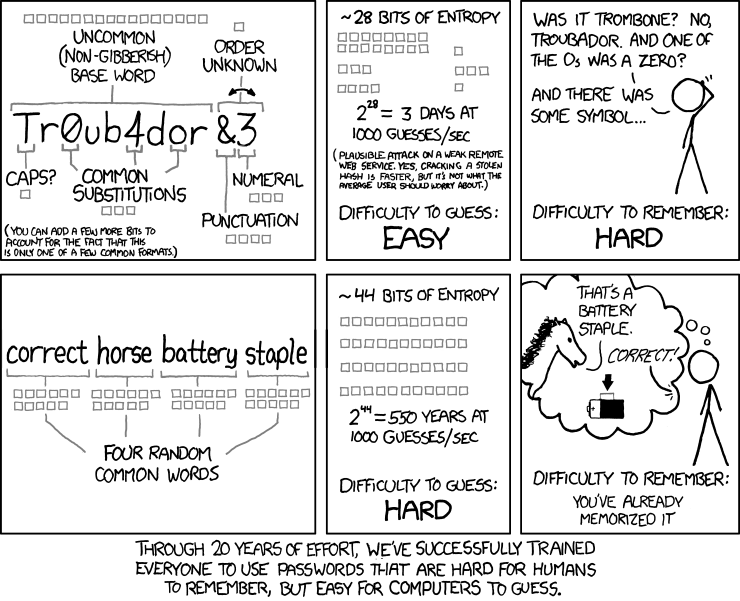
\includegraphics[width=\textwidth]{password_strength}
    \caption{Παράδειγμα Κωδικού με Συνδυασμό Λέξεων \label{fig:xkcd_password_strngth}}
\end{figure}

Προτείνεται επίσης να αποφεύγεται η επαναχρησιμοποίηση κωδικών, καθώς αν ο κωδικός σας διαρρεύσει από μία σελίδα, μπορεί να τοποθετηθεί σε ένα λεξικό με κωδικούς, και έπειτα να δοκιμασθεί και σε άλλες σελίδες.

Αποφύγετε επίσης να χρησιμοποιείτε στοιχεία σας, τα οποία είναι γνωστά σε τρίτους, όπως ονόματα κατοικίδιων ή μελών της οικογένειάς σας, ημερομηνίες γέννησης ή επετείους και προσωπικά στοιχεία όπως αριθμούς τηλεφώνων ή αστυνομικής ταυτότητας.

Συνοψίζοντας:

\begin{itemize}
    \item Χρησιμοποιήστε κωδικούς με μήκος τουλάχιστον 12 με 14 χαρακτήρες.
    \item Χρησιμοποιήστε κεφαλαίους και μικρούς χαρακτήρες, νούμερα, και ειδικούς χαρακτήρες αν επιτρέπεται.
    \item Παράγετε τους κωδικούς σας τυχαία όπου μπορείτε.
    \item Αποφύγετε την επαναχρησιμοποίηση κωδικών.
    \item Αποφύγετε εύκολους κωδικούς που προκύπτουν από μονοπάτια στο πληκτρολόγιο (π.χ. \texttt{asdf}), λέξεις που βρίσκονται αυτούσιες σε λεξικά (π.χ. \texttt{football}), αριθμητικές ακολουθίες (π.χ. \texttt{123789654}) και προσωπικά στοιχεία (π.χ. \texttt{17051994}).
\end{itemize}

\printbibliography[heading=bibintoc]

\end{document}
